\documentclass[12pt, a4paper]{article}
\usepackage[T2A]{fontenc}
\usepackage[utf8x]{inputenc}
\usepackage[english, russian]{babel}
\usepackage{mathtools}
\DeclareMathOperator{\arcsinh}{arcsinh}
\DeclareMathOperator{\arccosh}{arccosh}
\DeclareMathOperator{\arctanh}{arctanh}
\DeclareMathOperator{\arccoth}{arccoth}
\begin{document}
\title{Производная туда сюда
}\author{Севсоль, 1 курс ЭРТЭ}
\date{\today}
\maketitle 
\centerline{Ща производную такой вот функции за яйца возьмём}
\begin{equation}
f(x) = \frac{\arctan(x) \cdot \sinh({x}^{2})-\sqrt{{x}^{2}}}{\sinh(\cosh(\ln(x)))}
\end{equation}
\begin{center}
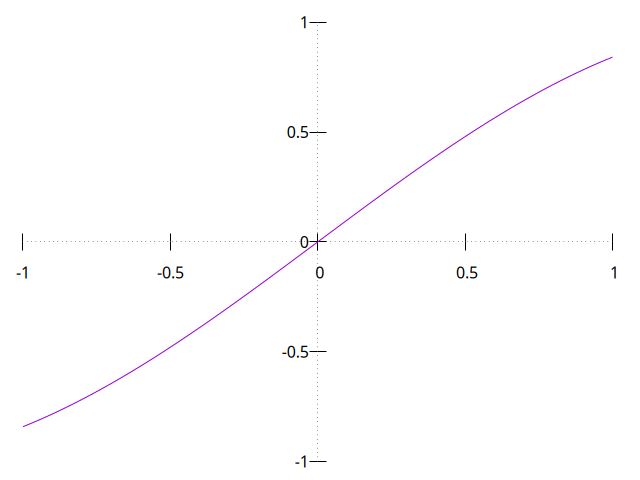
\includegraphics[scale=0.5]{start_func.png}
\end{center}
Очевидно, что
\begin{equation}
\frac{d}{dx}(x) = 1
\end{equation}
Согласано предложению 1488 Знаменской Люмдмилы Николаевны
\begin{equation}
\frac{d}{dx}(\arctan(x)) = \frac{1}{1+{x}^{2}}
\end{equation}
Люблю кафедру общесоса
\begin{equation}
\frac{d}{dx}(x) = 1
\end{equation}
Вам пора задуматься об обучении на Физтехе
\begin{equation}
\frac{d}{dx}(2) = 0
\end{equation}
Вам пора задуматься об обучении на Физтехе
\begin{equation}
\frac{d}{dx}(x) = 1
\end{equation}
Упростим
\begin{equation}
{x}^{1} = x
\end{equation}
Упростим
\begin{equation}
1x = x
\end{equation}
Очевидно, что
\begin{equation}
\frac{d}{dx}({x}^{2}) = 2x
\end{equation}
Люблю кафедру общесоса
\begin{equation}
\frac{d}{dx}(\sinh({x}^{2})) = \cosh({x}^{2}) \cdot 2x
\end{equation}
Я устал
\begin{equation}
\frac{d}{dx}(x) = 1
\end{equation}
Вам пора задуматься об обучении на Физтехе
\begin{equation}
\frac{d}{dx}(2) = 0
\end{equation}
Каждый советский дошкольник знает
\begin{equation}
\frac{d}{dx}(x) = 1
\end{equation}
Упростим
\begin{equation}
{x}^{1} = x
\end{equation}
Упростим
\begin{equation}
1x = x
\end{equation}
Каждый советский дошкольник знает
\begin{equation}
\frac{d}{dx}({x}^{2}) = 2x
\end{equation}
Вам пора задуматься об обучении на Физтехе
\begin{equation}
\frac{d}{dx}(\sqrt{{x}^{2}}) = \frac{2x}{2 \cdot \sqrt{{x}^{2}}}
\end{equation}
Вам пора задуматься об обучении на Физтехе
\begin{equation}
\frac{d}{dx}(\sinh({x}^{2})-\sqrt{{x}^{2}}) = \cosh({x}^{2}) \cdot 2x-\frac{2x}{2 \cdot \sqrt{{x}^{2}}}
\end{equation}
Блять завтра семестровая
\begin{equation}
\frac{d}{dx}(A) = C
\end{equation}
$$A = \arctan(x) \cdot \sinh({x}^{2})-\sqrt{{x}^{2}}$$
$$C = \frac{1}{1+{x}^{2}} \cdot \sinh({x}^{2})-\sqrt{{x}^{2}}+B$$
$$B = \cosh({x}^{2}) \cdot 2x-\frac{2x}{2 \cdot \sqrt{{x}^{2}}} \cdot \arctan(x)$$
Методом пристального взгляда
\begin{equation}
\frac{d}{dx}(x) = 1
\end{equation}
Люблю кафедру общесоса
\begin{equation}
\frac{d}{dx}(\ln(x)) = \frac{1}{x}
\end{equation}
Методом пристального взгляда
\begin{equation}
\frac{d}{dx}(\cosh(\ln(x))) = \sinh(\ln(x)) \cdot \frac{1}{x}
\end{equation}
Методом пристального взгляда
\begin{equation}
\frac{d}{dx}(\sinh(\cosh(\ln(x)))) = D
\end{equation}
$$D = \cosh(\cosh(\ln(x))) \cdot \sinh(\ln(x)) \cdot \frac{1}{x}$$
Уважаемая КВМ, пососите мои яйки
\begin{equation}
\frac{d}{dx}(\frac{A}{\sinh(\cosh(\ln(x)))}) = \frac{C \cdot \sinh(\cosh(\ln(x)))-D \cdot A}{{\sinh(\cosh(\ln(x)))}^{2}}
\end{equation}
$$A = \arctan(x) \cdot \sinh({x}^{2})-\sqrt{{x}^{2}}$$
$$C = \frac{1}{1+{x}^{2}} \cdot \sinh({x}^{2})-\sqrt{{x}^{2}}+B$$
$$B = \cosh({x}^{2}) \cdot 2x-\frac{2x}{2 \cdot \sqrt{{x}^{2}}} \cdot \arctan(x)$$
$$D = \cosh(\cosh(\ln(x))) \cdot \sinh(\ln(x)) \cdot \frac{1}{x}$$
$$A = \arctan(x) \cdot \sinh({x}^{2})-\sqrt{{x}^{2}}$$


Вот мы и посчитали производную. Кстати, уважаемая КВМ, пососите мои яйки.

\end{document}
